\documentclass{article}
\usepackage{graphicx}
\usepackage[margin=1.5cm]{geometry}
\usepackage{amsmath}

\begin{document}

\title{Monday Reading Assessment: Unit 1, Gauss' Law}
\author{Prof. Jordan C. Hanson}

\maketitle

\section{Gauss' Law}

\begin{enumerate}
\item Observe Fig. \ref{fig:spheres1}.  This question is about objects with spherical symmetry.
\begin{figure}[ht]
\centering
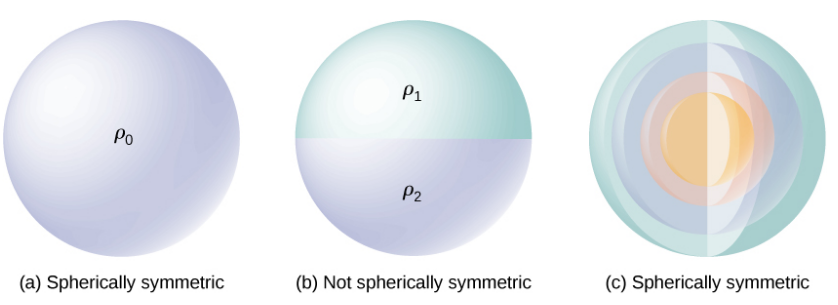
\includegraphics[width=0.35\textwidth]{spheres.png}
\caption{\label{fig:spheres1} Charge distributions with (a) spherical symmetry (b) no spherical symmetry (c) spherical symmetry.}
\end{figure}
Which of the following charge distributions has \textit{spherical} symmetry?
\begin{itemize}
\item A: A long line of charge, uniformly spread in one dimension
\item B: A disk of charge, evenly spread in two-dimensions
\item C: A point charge
\item D: A shell of charge with radius $R$, evenly spread over the shell
\end{itemize}
Which of the following charge distributions has \textit{spherical} symmetry?
\begin{itemize}
\item A: A sphere of charge, with positive charge out to a radius $r$, then negative charge out to a radius $R$
\item B: A sphere of charge, with positive charge on one hemisphere, and negative charge on the other hemisphere
\item C: A sphere of charge, with positive charge from $0 \leq \phi < \pi/2$, negative charge from $\pi/2 \leq \phi < \pi$, positive charge from $\pi \leq \phi < 3\pi/2$, and negative charge from $3\pi/2 \leq \phi < 2\pi$
\item D: A shell of charge with radius $R$, with random charge density
\end{itemize}
\item Use Gauss' law to show that (a) the E-field a distance $r$ from a point charge $Q$ is $E = Q/\left(4\pi \epsilon_0 r^2\right)$.  (b) Show that the E-field a distance $r$ from the origin inside a uniformly charged sphere with charge density $\rho$ and radius $R$ that is centered at the origin is a linear function of $r$.  \textit{Hint: draw the sphere, and then draw a shell of radius $r$ with $r<R$.  How much charge is enclosed?} (c) Far outside the sphere, how does the E-field depend on $r$?  \textit{Hint: this is true for anything, if you are far enough away.}
\end{enumerate}

\end{document}
